% -*- mode: latex; fill-column: 65; -*-
\documentclass[aps, pra, preprint]{revtex4-1}
\usepackage{todonotes}
\usepackage{amssymb}
\usepackage{amsmath}
\usepackage{siunitx}

\bibliographystyle{apsrev4-1}

\newcommand{\hfree}{H_{\rm free}}
\newcommand{\phicap}{\varphi_{\rm cap}}
\newcommand{\phiwall}{\varphi_{\rm wall}}


\begin{document}

\title{Computational analysis of laser cooling of ultra-cold ions
  in Penning traps
}

\author{Dominic Meiser}
\affiliation{Trimble Inc, Boulder, 4730 Walnut Street, Suite 201,
Boulder, CO 80301, USA.}
\author{John J Bollinger}
\affiliation{National Institute of Standards and Technology,
Boulder, Colorado 80305, USA.}

\begin{abstract}
  Here goes the abstract.
  \todo{Write abstract}
\end{abstract}

\maketitle


Ultra-cold ions in Penning traps are an experimental system that
enable many studies at the forefront of quantum science and
condensed matter physics. For many of these studies it is
beneficial to prepare the ultra-cold ion ensemble in the coldest
state possible. For example, for quantum
metrology\todo{references} and quantum simulation
experiments\todo{references}, cold temperatures enable single
site optical access to individual ions for precise state
preparation and high fidelity state readout. In squeezing
experiments colder temperatures can reduce dephasing rates.

{\bf For what types of experiments for are colder temperatures
beneficial?}
\begin{itemize}
\item Metrology and squeezing experiments
\item Quantum simulation experiments, Ising
  model\cite{Britton:EngineeredIsingModel}, quantum magnetism,
  condensed matter, etc.
\item Quantum information and quantum computing? Is that within
  reach for Penning trap experiments?
\end{itemize}k

{\bf How do these experiments benefit from cold temperatures?}
\begin{itemize}
\item Improved crystal stability
\item Longer interrogation times
\item Higher fidelity state preparation
\item Smaller dephasing rates
\item Higher precision/fidelity state readout
\item single site access
\end{itemize}

{\bf How are cold temperatures achieved?} The primary means of
cooling ions in Penning traps are various forms of laser cooling
including Doppler cooling and side band cooling. While the basic
principles of laser cooling for ultra-cold ions is the same as
for neutral atoms in magneto-optical traps there are also
significant differences that can make it challenging to
understand the experimentally achieved ion temperature, cooling
limits, cooling and heating mechanisms, and that can make it more
challenging to optimize the cooling laser parameters such as
intensity and detuning as well as the cooling laser geometry.

{\bf What is different and more challenging for ions compared to
neutral atoms?} A major difference compared to neutral atom
experiments is that ions in Penning traps move in a magnetic
field several Tesla strong. The Lorentz force in the magnetic
field forces the ions into circular orbits with a cyclotron
frequency on the order of a few hundred kilo Hertz. The rotation
of the ions in the magnetic field means that the ions velocity
periodically changes direction relative to any cooling laser
beams that are stationary in the laboratory frame of reference. A
second major difference is the strong interaction between the
ions due to the Coulomb force. The Coulomb force couples the ions
into collective modes of motion. In contrast to the cooling
dynamics of neutral atoms---which is largely a single particle
phenomenon---it is necessary to take the collective nature of the
ion motion into account to fully understand the cooling dynamics
of ultra-cold ions in Penning traps.

{\bf What do we contribute in this paper?} To help us better
understand the dynamics of ultra-cold ions in Penning traps we
have developed computer simulations that allow us to
quantitatively track the dynamics of the ions over time scales
from fractions of a nano-second all the way to milli seconds and
seconds. In this paper we demonstrate the validity of these
simulations by comparison with other simulations as well as by
comparison with experimental data. We then use these simulations
to study the spectra of the out-of-plane and in-plane modes of
motion of ultra-cold ions. We compute the temperatures of these
modes and determine optimal laser cooling parameters.

{\bf Who has studied cooling dynamics before? How did they do
it?} Need a significant review of the existing literature here.
Some key workds: Dan Dubin, Dave Wineland and JJ Bollinger,
Molecular Dynamics simulations, analytical studies, fluid models,
tracking codes, particle methods, PIC, Direct Simulation Mode
Carlo (DSMC).

{\bf What will we discuss in the rest of this paper}


\section{Model and computational algorithm}

In this section we describe our mathematical model as well as the
computational techniques used in our simulations.


\subsection{Mathematical model}

We treat the ions as classical point like particles with 
velocity $\mathbf{v}_i$ and position $\mathbf{x}_i$. The motion
of the ions is governed by the Hamiltonian
\begin{equation}
  H = \hfree + \sum_{i=1}^N q_i\varphi(\mathbf{x}_i)\;,
\end{equation}
where the free Hamiltonian
\begin{equation}
  \hfree =
  \sum_{i=1}^N \frac{1}{2m_i}\left(
    \mathbf{p}_i -
    q_i\mathbf{A}(\mathbf{x}_i) \right)^2 
\end{equation}
includes the vector potential $\mathbf{A}$ corresponding to the
axial magnetic field in the Penning trap, $\mathbf{B} =
\mathbf{\nabla}\times \mathbf{A}$, parallel to the $z$ axis. In
these equations $N$ is the number of ions in the trap, $m_i$ is
the mass of ion $i$, $q_i$ its charge, and the electrostatic
potential
\begin{equation}
  \varphi(\mathbf{x}_i) =
  \phicap(\mathbf{x}_i) +
  \phiwall(\mathbf{x}_i) +
  \sum_{\substack{j=1\\j\neq i}}^N
  \frac{1}{4\pi\varepsilon_0}\
  \frac{q_j}{\left| \mathbf{x_i} - \mathbf{x_j} \right|}
\end{equation}
contains the potential $\phicap$\todo{Need discussion of
$\phicap$} due to the end-cap electrodes in the Penning trap,
the rotating wall potential $\phiwall$, and the Coulomb potential
for the interaction between the ions.

In addition to the conservative dynamics described by the
Hamiltonian the ions are subject to radiation pressure forces due
the cooling lasers. We describe the radiation pressure force
using a stochastic model. We discuss this model in more detail
when we consider the computational integration of the ion motion
in the next section.


\subsection{Numerical algorithm}

To numerically integrate the motion of the ions we employ a split
step algorithm as is customary in e.g. molecular dynamics
simulations. To advance the positions and velocities of the ions
$\{\mathbf{x}_i, \mathbf{p}_i\}$
from time $t$ to $t + \Delta t$ we use the update formula
\begin{equation}
  \{\mathbf{x}_i, \mathbf{p}_i\}(t+\Delta t) =
  U_{\rm free}(\Delta t /2)
  U_{\rm kick}(t + \Delta t / 2; \Delta t)
  U_{\rm free}(\Delta t /2)
  \{\mathbf{x}_i, \mathbf{p}_i\}(t)\;.
\end{equation}
In this formula, $U_{\rm free}(\Delta t/2)$ is the time evolution
operator corresponding to the $\hfree$ that advance the state of
the ions for a time interval of duration $\Delta t / 2$. Since
the free Hamiltonian contains just the kinetic energy of the ions
and the Lorentz force due to the axial magnetic field the motion
generated by $U_{\rm free}$ is the well known circular Larmor
precession,
\todo{Formulas for drift along $z$ and circular motion in $x-y$
plane.}
\begin{eqnarray}
  \mathbf{x}_i &= \ldots\\
  \mathbf{p}_i &= \ldots
\end{eqnarray}
The time evolution operator $U_{\rm kick}(t + \Delta t/2; \Delta
t)$ corresponds to the interaction with the forces due to the
electrostatic potential as well as the radiation pressure forces
due to laser cooling. This operator is time dependent due to the
rotating wall potential and the radiation pressure forces. We
evaluate it at the mid-point of the time interval, $t + \Delta t
/ 2$. The operator $U_{\rm kick}$ changes the momenta of the
particles only,
\begin{eqnarray}
  \{\mathbf{x}_i, \mathbf{p}_i\}(t + \Delta t)
  &=& U_{\rm kick}(t + \Delta t /2; \Delta t)
    \{\mathbf{x}_i, \mathbf{p}_i\}(t)\\
  &=&\left\{
      \mathbf{x}_i(t),
      \mathbf{p}_i(t) +
      \Delta t q_i \mathbf{E}(t + \Delta t / 2, \mathbf{x}_i) +
      \Delta \mathbf{p}_i^{\rm laser}
      \right\}\;.
\end{eqnarray}
The kick due to the electric field is given by $\Delta t
q_i\mathbf{E}(t+\Delta t /2,\mathbf{x}_i) = -\Delta t
q_i\mathbf{\nabla}\varphi(\mathbf{x}_i)$.

The radiation pressure forces due to the laser cooling lead to
the momentum kick $\Delta \mathbf{p}_i^{\rm laser}$. To find this
kick we Find the number $n_{\rm scattered}$ of photons scattered
based on velocity and intensity at location of ion in time
interval $\Delta t$ (Doppler shift, saturated two level resonance
fluorescence, Poisson distributed)\todo{Discuss scattering
rates}, find $n_{\rm scattered}$ directions isotropically
distributed. This is only approximately correct as the scattering
pattern is not isotropic in reality. And then we find the
momentum kick as
\begin{equation}
\Delta \mathbf{p}_i^{\rm laser} = n_{\rm scattered}\hbar
\mathbf{k} + \sum_{i=1}^{n_{\rm scattered}} \hbar \mathbf{k}_i\;.
\end{equation}
\todo{Discuss limitations of this approach. Low saturation.}

In the absence of laser cooling the integration formula is
symplectic. This means that the integrator is long term stable
and has the qualitatively correct behavior. However, the laser
cooling terms break the symplecticity because the cooling force
depends both on the positions of the ions and their momenta.


\subsection{Convergence}

One of the most basic tests of the correctness of our time
integration scheme is to verify that it converges to a solution
as the time step size is reduced. To evaluate the convergence we
initialize our simulation with a steady state configuration of
127 ions shown in Fig.~\ref{fig:initial_state_top_view}. Here and
in the results discussed below we use parameters typical for the
Penning trap at NIST Boulder with a homogeneous magnetic field of
$B=\SI{4.4588}{\tesla}$,
a trap rotation frequency of $\omega_{\rm trap}=2\pi\times
\SI{180}{\kilo \hertz}$, end cap voltages yielding a confining
potential of $k_z=\ldots$\todo{What are the units here?}, and a
rotating wall potential of $V_{\rm Wall} = \SI{1}{\volt}$
yielding $\delta=\SI{3.5e-4}{}$.
\begin{figure}
  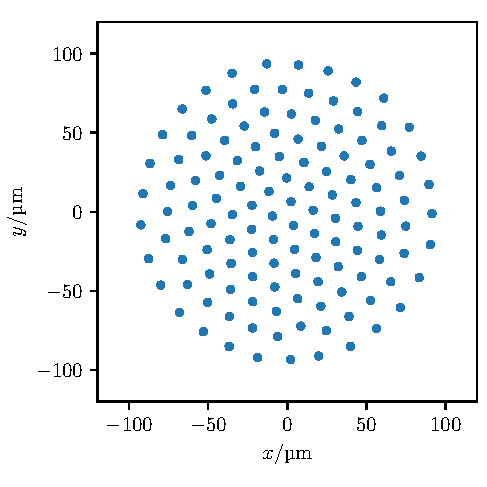
\includegraphics{./figures/fig_initial_state_top_view.pdf}
  \caption{Top view of steady state configuration of ions in
    Penning trap used for convergence study.}
  \label{fig:initial_state_top_view}
\end{figure}

Starting from this initial steady state configuration we
integrate the equations of motion for $\SI{10}{\us}$ using
different time step sizes. For each time step size we compare the
final solution with a reference solution computed using a time
step size of $\Delta t = \SI{2e-10}{\second}$. We compute the
error $\Delta x(\Delta t)$ in the simulation result
$\mathbf{x}(\Delta t)$ as the average Euclidian distance between
the reference solution $\mathbf{x}^{\rm
  ref}=\mathbf{x}(\SI{2.0e-10}{\second})$,
\begin{equation}
  \Delta x(\Delta t) =
  \sqrt{N^{-1}\sum_{i=1}^N\left(
      \mathbf{x}_i(\Delta t)-\mathbf{x}_i^{\rm ref}\right)^2}\;.
\end{equation}

The result is shown in Fig.~\ref{fig:convergence}. The error
decreases quadratically for time step sizes below approximately
$\SI{1.0e-7}{\second}$. At time step size of $\Delta t =
\SI{1}{\nano\second}$ the mean position error of the ions is
$\Delta x(\SI{1}{\nano\second})\approx \SI{1}{\nano\meter}$. For
reference, during this time interval the ions move on the order
of $\SI{1}{\milli\meter}$, i.e. the ion motion is integrated with
a relative error on the order of $\SI{1.0e-6}{}$. For time step
sizes greater than $\Delta t\approx 1.0e-7$ the integrator can be in
resonance with some of the vibrational eigen modes of the system.
Whenever the integrator is in resonance errors can grow
indefinitely. While damping forces such as laser cooling can
broaden the resonances and limit the growth of errors it is best
to stick to time step sizes that are smaller than $\Delta t =
\SI{1.0e-7}{\second}$. Results quoted in this paper were obtained
with $\Delta t = \SI{1}{\nano\second}$ unless noted otherwise.
\begin{figure}
  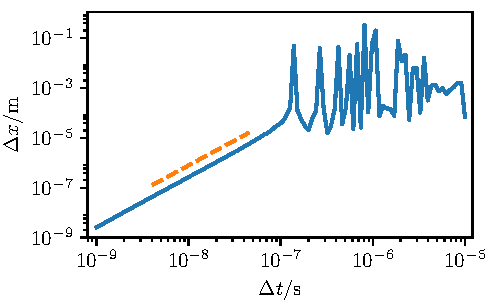
\includegraphics{./figures/fig_convergence.pdf}
  \caption{Integration errors as a function of time step size for
    a total time integration time of $T=\SI{10}{\us}$ for a
    typical Penning trap simulation. The dashed orange line is a
    quadratic for orientation. See text for details.}
  \label{fig:convergence}
\end{figure}


\section{Single-plane to multi-plane instability}


\section{Finite temperature mode analysis}

\subsection{Out-of-plane modes}

\subsection{In-plane modes}



\section{Conclusion}

\bibliography{cooling_bibliography}

\end{document}
